\documentclass{report}
\usepackage{homework}
\solstrue

\usepackage{graphicx}
\graphicspath{{figures/}}

\renewcommand{\hmwkTitle}{Homework 5}

\begin{document}
\mktitle

\begin{problem}

\begin{figure}[!ht]
	\centering
	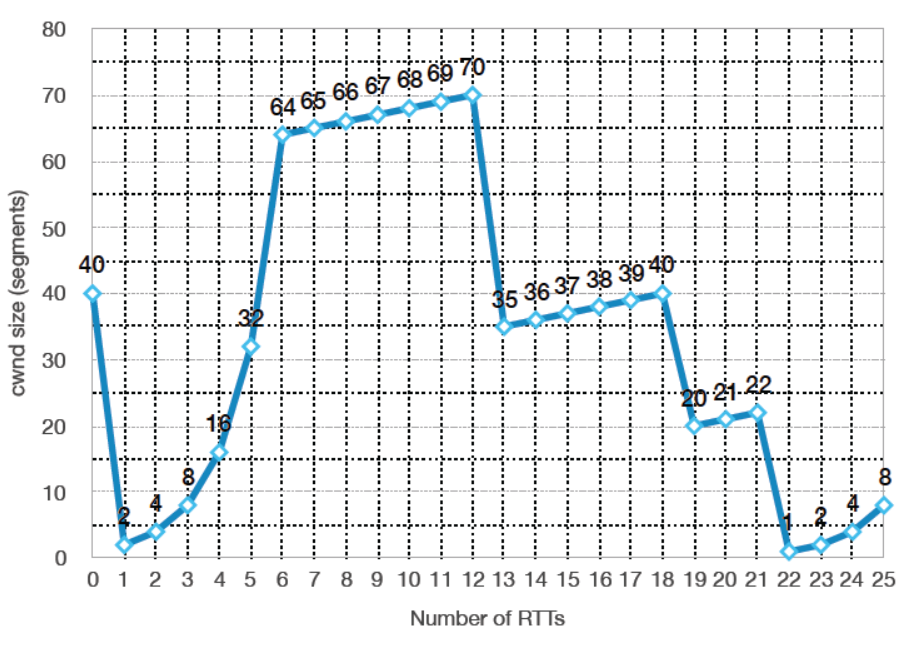
\includegraphics[width=0.7\textwidth]{hw5_fig1.png}
	\caption{TCP congestion control.}
	\centering
	\label{fig:image2}
\end{figure}

Assume that a TCP connection has been running between hosts A and B for sometime, so that the number of RTTs shown in the above graph are with respect to the time when you started observing the the cwnd value of this connection.  Hosts A and B use TCP Reno (with Fast Retransmit and Fast Recovery). 

\begin{enumerate}
\item \textbf{On the graph above}, identify the time periods when TCP slow start is operating.
\item \textbf{On the graph above}, identify the time periods when TCP congestion avoidance is operating (AIMD).
\item For each loss event, specify whether it was detected by a triple duplicate ACK or by a timeout
\item For each loss event, indicate the value of the slow start threshold (ssthresh)
\end{enumerate}

\begin{answer}{22em}
    Write your answer here
\end{answer}

\end{problem}



\newpage



\begin{problem}
Assume that host A sets up a TCP connection with host B to send data. Assume that A's \texttt{ssthresh} value is 64 KB and TCP segment size is 3 KB.
\begin{enumerate}
	\item How many bytes have been transmitted after 3 RTTs assuming no losses? Show your work.
	\item Now, suppose that after the third RTT, a loss occurs which results in the TCP sender's retransmission timer to expire. What actions will TCP congestion control take in this case?
	\item Assuming no further packet loss occurs from then on, how many RTTs does it take to transmit an additional 22 KB of data?
\end{enumerate}


\begin{answer}{35em}
  Write your answer here
\end{answer}

\end{problem}


\newpage



\begin{problem}
True or False? Briefly explain your answer in a single sentence.

\begin{enumerate}
    \item Host A is sending Host B a large file over a TCP connection. Assume Host B has no data to send Host A. Host B will not send acknowledgments to Host A because Host B cannot piggyback the acknowledgments on data.
    \item  The size of the TCP \textit{rwnd} never changes throughout the duration of the connection.
    \item  Suppose Host A is sending Host B a large file over a TCP connection. The number of unacknowledged bytes that A sends cannot exceed the size of the receive buffer.
    \item  Suppose Host A is sending a large file to Host B over a TCP connection. If the sequence number for a segment of this connection is m, then the sequence number for the subsequent segment will necessarily be m + 1.
    \item  The TCP segment has a field in its header for \textit{rwnd}.
    \item  Suppose that the last SampleRTT in a TCP connection is equal to 1 sec. The current value of TimeoutInterval for the connection will necessarily be $\geq$ 1 sec.
    \item  Suppose Host A sends one segment with sequence number 38 and 4 bytes of data over a TCP connection to Host B. In this same segment the acknowledgment number is necessarily 42.
\end{enumerate}


\begin{answer}{35em}
  Write your answer here
\end{answer}

\end{problem}

\newpage



\begin{problem}

As we have discussed in the class, a timer is a useful component in various protocol designs: because a communicating end cannot see what is going on either inside the network or at the other end, when needed it sets up an "alarm", and takes some action when the alarm goes off.

\begin{enumerate}
    \item Does HTTP use any timers? If so, please briefly describe how each is used. If not, please explain why it does not need one.
    \item Does DNS use any timers? If so, please briefly describe how each is used. If not, please explain why it does not need one.
    \item Does TCP use any timer?  If so, please briefly describe how each is used. If not, please explain why it does not need one.
    \item Does UDP use any timer?   If so, please briefly describe how each is used. If not, please explain why it does not need one.
\end{enumerate}

\begin{answer}{40em}
    Write your answer here
\end{answer}

\end{problem}

\end{document}
